\appendix

\section{Database Design}

\begin{figure}[tbh]
\centering
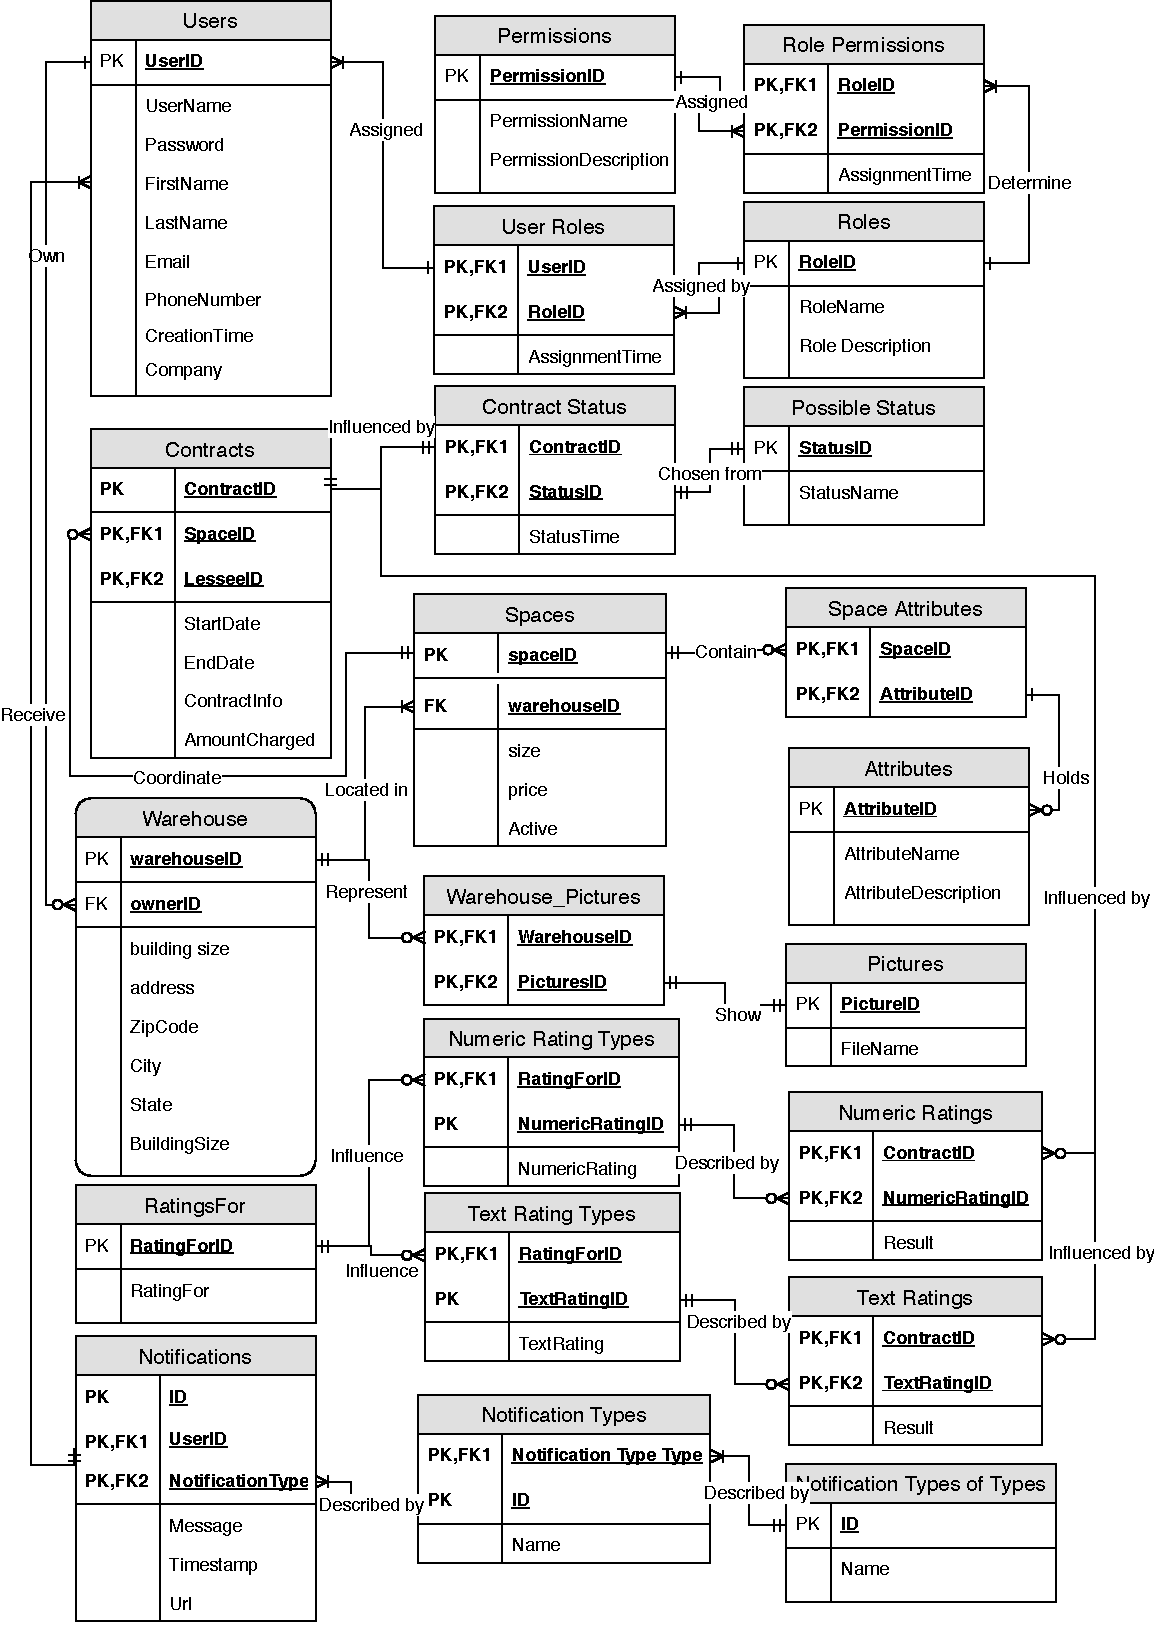
\includegraphics[page=1,width=.85\textwidth,height = .7\textheight]{Phase_3/ER_Diagram.pdf} 
\caption{Entity-Relationship Diagram}
\end{figure}

\pagebreak
\section{Ranking Algorithm}

\subsection{Utilization}
The ranking algorithm's dependency on utilization considers all the previous and future contracts for a designated space.  Utilization is divided into two parts, future utilization and past utilization.  The utilization equation is displayed in Equation~\ref{fig:utilization}.  This equation take the proportion between the time until or since the contract over the length of the contract.  This strategy promotes spaces that have not had a contract in a long time, and spaces that have shorter contracts.  Therefore the algorithim distributes contracts to a greater portion of the @Capacity community because this algorithm will distribute a higher score to less used space spaces.


\begin{figure}[h]
\[\text{Utilization} = \frac{\text{Time Until or Since the Contract}}{\text{Contract Length}}\]
\caption{Utilization for Contracts}
\label{fig:utilization}
\end{figure}


\subsection{Score}

The total score used by the ranking algorithm is a composite of 4 scores: distance, price, utilization and size.  Each one of these scores has an associated scale factor that can be changed based on the importance of each factor.  By default all the scores are scaled the same.  The total score is a simple weighted addition of each of the 3 factors as described below.



\subsubsection{Distance}

The distance score is calculated on line 287-297 in the "www/includes/rankingFunctions.php" file.  Distance\textunderscore away is a measure of how far away a given warehouse is from the clients given location.  Max\textunderscore distance\textunderscore wanted is maximum distance away a client wants their potential warehouse.  The equation below gives a linearly decreasing score to each warehouses based on its distance from the client defined location.  

\begin{figure}[h]
\[\mathrm{distance\_ score\ }=\mathrm{\ scale\ }\ast\ \left(1\ -\ \frac{(\mathrm{distance\_ away})}{(\mathrm{max\_ distance\_ wanted})}\right)\]
\caption{Distance ranking score}
\label{fig:dist}
\end{figure}

\subsubsection{Price}

The price score is calculated on line 322-326 in the "www/includes/rankingFunctions.php" file.  Space\textunderscore price is the cost of a given space.  Min\textunderscore price is the price of the cheapest space that fits the client's needs.  Max\textunderscore price is the price of the most expensive space that fits the client's needs.  The equation below gives the most expensive warehouse a score of 0, the least expensive a score of 1, and every warehouse in between a linear score between 0 and 1.

\begin{figure}[h]
\[\mathrm{price\_ score}\ =\mathrm{\ scale\ }\ast\left(1\ -\ \frac{\left(\mathrm{space\_ price\ }-\mathrm{\ min\_ price}\right)}{\left(\mathrm{max\_ price}\ -\ \mathrm{min\_ price}\right)}\right)\]
\caption{Price ranking score}
\label{fig:price}
\end{figure}

\subsubsection{Size}
The size score is calculated on line 299-320 in the "www/includes/rankingFunctions.php" file. Space\textunderscore score is the score given for each space in a warehouse. Max\textunderscore size represents the max size that each individual space has available for rent. Space\textunderscore size is user inputted value for their desired space size. This equation gives a linearly decreasing score to each warehouses based on its difference from the lessee defined size.  

\begin{figure}[h]

\[\mathrm{size\_ score}\ =\text{scale} * (1-\frac{\text{SpaceSize} - \text{SizeWanted}}{\text{MaxSpaceSize}})\]
\caption{Size ranking score}
\label{fig:size}
\end{figure}
\newpage
\section{Synthetic Data Generation}

\textbf{Contracts Pseudocode}
\\The code pertaining to the following pseudocode can be found on lines 302-362 on the file FINAL DATA GENERATION.R within the dataGeneration folder
\begin{enumerate}
\item Designate how many contracts are to be generated.
\item Generate a random number between 1 and 1400 (1400 being the number of spaces) to assign a space ID to each contract that is to be generated. 
\item Generate a random number between 350 and 1000 (this range being the range of lessee user IDs) to assign a lessee ID to each contract that is to be generated. The reason the random number is generated between 350 and 1000 is because 400-1000 are lessee user IDs, 1-350 are owner IDs, and 350-400 is a mixture of lessee and owner IDs.
\item Sort all space IDs in increasing order.
\item For each contract, if the current space ID is equal to the previous space ID, set the contract's start date equal to a random date that is greater than or equal to the previous contract's end date.
\item If the current space ID is different than the previous space ID, set the current contract's start date to a random date.
\item Set the end date for each contract to a date greater than the start date by a random number of days ranging from two weeks to two years.
\item Calculate the amount charge: for each contract, multiply the space's price/square foot/month by the length of the contract in months, the space's size, and the service fee.
\item Generate the contract information for each contract by pulling one string of random storage information from a list of storage items.
\item Compile the space ID, lessee ID, start date, end date, amount charged, and contract information into a data frame.
\item Write the contract data to a CSV file
\end{enumerate}
An important aspect to synthesizing random data that is also realistic is creating realistic contracts, as contracts are the entity that tie the space and lessee together. A realistic contract is a contract that is assigned to a particular space and lessee, does not overlap with another contract in the same space, lasts for a reasonable time, has a price calculated based on size and time, and contains information on what is being store. For this data, each contract is assigned to a space and lessee randomly using a simple "sample" function over the range of possible values for each attribute. The price is calculated using the space price and space size calculated during the space data generation. In this case, it was important to ensure that the price and size that were being used in each contract's price calculation corresponded to the space that the contract was being assigned to.\\
\\Another extremely important issue in creating realistic contracts was the scheduling aspect. As previously stated, realistic contract data contains start date and end dates that do not overlap for the same space. In order to prevent this from happening, the same logic that was used in the scheduling algorithm was applied to creating this data. This entails checking to see if a proposed contract's start date is before an existing contract's end date. In essence, this means contracts do not get assigned to spaces with outstanding contract requests. 

